\documentclass{article}
%\usepackage{geometry}
%\usepackage[hmargin={3cm,3cm},vmargin={2.5cm,2.5cm},marginparsep=2mm,showframe]{geometry} % shows frame
\usepackage[hmargin={3cm,3cm},vmargin={2.5cm,2.5cm},marginparsep=2mm]{geometry}
%\usepackage[showframe,pass]{geometry}  % shows frame but does not change page geometry

%\usepackage{ametsoc}
\usepackage[intlimits]{amsmath}
\usepackage{bm}
%\usepackage{amssymb,latexsym,graphics}
\usepackage{natbib}  % all options handled by \bibstyle@XXX below

\usepackage{booktabs}
%\usepackage[notcite,notref]{showkeys}
\usepackage[osf]{mathpazo} % palatino fonts % uncomment for Palatino font
\usepackage{todonotes}
%\usepackage[disable]{todonotes} % remove [disable] to see to-do notes
\usepackage{mdframed}
\mdfsetup{
backgroundcolor=yellow!20,
leftmargin=0.5cm,
leftline=false,
rightline=false
}
\definecolor{darkgreen}{rgb}{0,0.5,0}
\usepackage[linkcolor=blue,citecolor=darkgreen,colorlinks=true]{hyperref}
\usepackage{wrapfig}

\usepackage{siunitx}

% + custom commands - - - - - - - - - - - - - - - - - - - - - - - - - - - - - - - - - -
\newcommand{\pderiv}[2]{\frac{\partial #1}{\partial #2}} % partial derivative
\newcommand{\fderiv}[2]{\frac{d #1}{d #2}} % full derivative
\newcommand{\incr}[2]{\frac{\partial #1}{\partial #2}\Delta #2} % partial derivative

\title{Simulations with toy model of surface energy balance}

% + main body - - - - - - - - - - - - - - - - - - - - - - - - - - - - - - - - - - - - -
\begin{document}
\maketitle

We consider a simple system of energy fluxes shown in
Figure~\ref{figure:energy-balance}. For simplicity, we limit the consideration
to the fluxes of radiation and sensible heat, leaving evaporation and water
content aside. In this case, the equation for the two prognostic variables can
be written as follows:

\begin{align}
    C_a \fderiv{T_a}{t} &= S + H \\
    C_g \fderiv{T_g}{t} &= SW + LW - H
\end{align}
where
$C_a$ and $C_g$ are the heat capacities of the atmospheric layer and the ground,
$T_a$ and $T_g$ are the temperatures of the atmosphere and the ground,
$S$ is the heat input to the atmospheric layer (e.g. Newtonian nudging
toward prescribed temperature), positive to the layer;
$SW$ and $LW$ are the net short-wave and long-wave surface radiation,
\emph{both positive to the surface},
$H$ is the sensible heat flux, positive upwards.

\begin{wrapfigure}{R}{0.33\textwidth}
\centering
   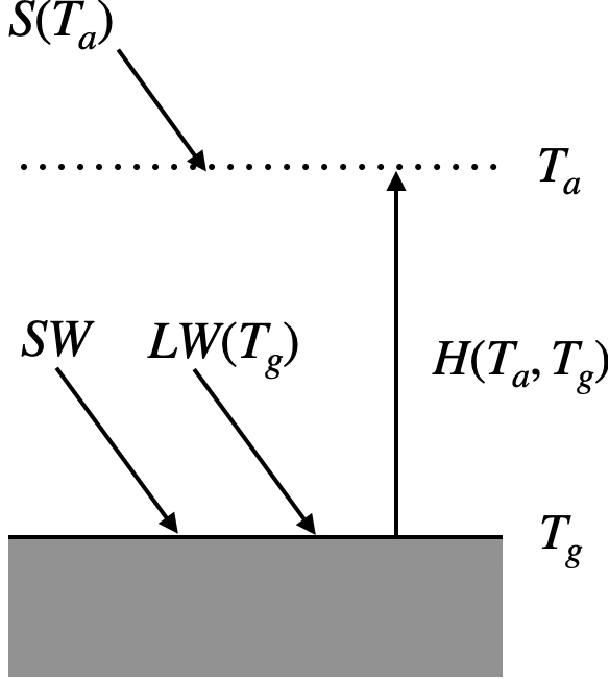
\includegraphics[width=0.32\textwidth]{energy-balance.pdf}
   \caption{Cartoon of the energy fluxes in the system}
   \label{figure:energy-balance}
\end{wrapfigure}

We assume that some energy terms depend on the state variables $T_a$ and $T_g$:
\begin{equation}
    H = H(T_g, T_a); \quad S = S(T_a); \quad LW = LW(T_g)
\end{equation}

Linearized and discretized:
\begin{align}
    \label{atm-eb-lin}
    C_a \frac{\Delta T_a}{\Delta t} &= S_0 + \incr{S}{T_a} + H_0 + \incr{H}{T_a} + \incr{H}{T_g} \\
    \label{sfc-eb-lin}
    C_g \frac{\Delta T_g}{\Delta t} &= SW + LW_0 + \incr{LW}{T_g} - H_0 - \incr{H}{T_a} - \incr{H}{T_g}
\end{align}

From equation~\eqref{atm-eb-lin}, moving all terms with $\Delta T_a$ to the left-hand side:
\begin{equation}
    \bigg( \frac{C_a}{\Delta t} - \pderiv{S}{T_a} - \pderiv{H}{T_a} \bigg) \Delta T_a =
        S_0 + H_0 + \incr{H}{T_g}
\end{equation}

In other words, we can express
\begin{equation}
    \label{fwd}
    \Delta T_a = f + e \Delta T_g
\end{equation}
where we introduce notation
\begin{align}
    f          &\equiv (S_0 + H_0) \Gamma^{-1} \\
    e          &\equiv \pderiv{H}{T_g} \Gamma^{-1} \\
    \Gamma     &\equiv \bigg( \frac{C_a}{\Delta t} - \pderiv{S}{T_a} - \pderiv{H}{T_a} \bigg)
\end{align}

Note that both $\pderiv{S}{T_a}$ and $\pderiv{H}{T_a}$ are negative, so that $\Gamma$
remains positive even id $C_a = 0$.

Likewise, from equation~\eqref{sfc-eb-lin} using notation from
equation~\eqref{fwd} we get
\begin{align}
    \bigg( \frac{C_g}{\Delta t} - \pderiv{LW}{T_g} + \pderiv{H}{T_g} \bigg) \Delta T_g
        & = SW + LW_0 - H_0 - \incr{H}{T_a} \\
        & = SW + LW_0 - H_0 - \pderiv{H}{T_a} \left( f + e \Delta T_g \right)
\end{align}

\begin{equation}
    \bigg( \frac{C_g}{\Delta t} - \pderiv{LW}{T_g} + \pderiv{H}{T_g} + \pderiv{H}{T_a} e \bigg) \Delta T_g
        = SW + LW_0 - H_0 - \pderiv{H}{T_a} f
\end{equation}

\end{document}